\documentclass[../../Main.tex]{subfiles}

\begin{document}
    \begin{figure}[hbt!]
        \centerline{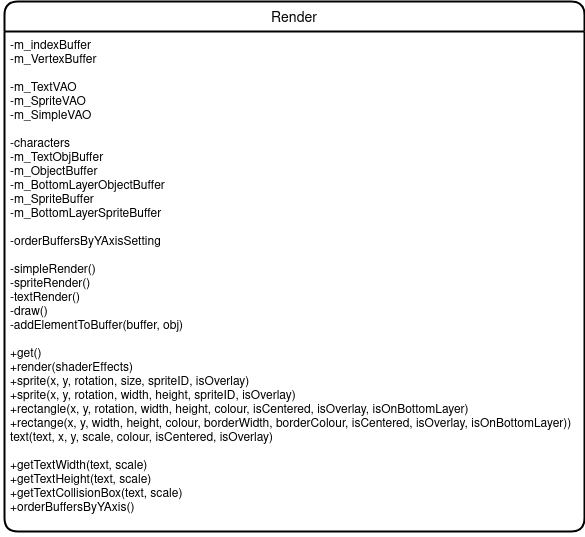
\includegraphics[scale=0.5]{img/Classes/Render.png}}
        \caption{Render class (singleton)}
        \label{fig}
    \end{figure}
    \begin{center}
        Variables
        \begin{tabular}{ | m{0.45\textwidth} | m{0.45\textwidth} | }
            \hline
            \textbf{Variable Name} & \textbf{Description} \\
            \hline
            m\_IndexBuffer & Stores the index buffer used for drawing all the vertices in the right order \\
            \hline
            m\_VertexBuffer & Stores the buffer used for all the rendering \\
            \hline
            m\_TextVAO & Stores the vertex array for drawing text \\
            \hline
            m\_SpriteVAO & Stores the vertex array for drawing sprites\\
            \hline
            m\_SimpleVAO & Stores the vertex array for drawing rectangles\\
            \hline
            characters & Stores all the characters textures and information needed to draw each character of a text font \\
            \hline
            m\_TextObjBuffer & Stores all the objects that need to be rendered in this frame \\
            \hline
            m\_ObjectBuffer & Stores all the objects that need to be rendered in this frame \\
            \hline
            m\_BottomLayerObjectBuffer & Stores all the objects that need to be rendered before anything else on this frame \\
            \hline
            m\_SpriteBuffer & Stores all the sprite objects that need to be rendered this frame \\
            \hline
            m\_BottomLayerSpriteBuffer & Stores all the sprite objects that need to be rendered before anything else on this frame \\
            \hline
            orderBuffersByYAxisSetting & Boolean that tells whether the buffers should be sorted by the Y position of objects \\
            \hline
            m\_SpriteShader & Stores the shader for rendering sprites \\
            \hline
            m\_TextShader & Stores the shader for rendering text \\
            \hline
            m\_SimpleShader & Stores the shader for rendering coloured rectangles \\
            \hline
        \end{tabular}
        Functions
        \begin{tabular}{ | m{0.2\textwidth} | m{0.3\textwidth}| m{0.4\textwidth} | }
            \hline
            \textbf{Function Name} & \textbf{Parameters} & \textbf{Description} \\
            \hline
            simpleRender & & Renders everything stored in m\_ObjectBuffer and m\_BottomLayerObjectBuffer \\
            \hline
            spriteRender & & Renders everything stored in sprite buffers \\
            \hline
            textRender & & Renders everything in m\_TextObjBuffer \\
            \hline
            draw & Takes in a VAO to render with & Draws all the vertices stored in m\_VertexBuffer onto the screen with a given VAO \\
            \hline
            addElementToBuffer & Takes in the buffer to add the object to and the object & Adds an object onto a buffer taking into account orderBuffersByYAxisSetting \\
            \hline
            get & & Returns the only instance of Render \\
            \hline
            render & Takes in a list of shaderEffects to apply to the shaders & Sets the shaderEffects to the shaders and then calls the other render functions \\
            \hline
            sprite & Takes in all the information needed for rendering (Can use a size or a specific value for the width and the height) & Adds TexturedObject object to the sprite buffers \\
            \hline
            rectangle & Takes in all the information to render a rectangle, a second function is made for rendering rectangles with a border & Adds ColouredObject to the object buffers \\
            \hline
            text & Takes all the information in to render text on the screen & Adds TextObject to the text buffer\\
            \hline
            getTextWidth & Takes in the text and the scale & Returns the width of a given text at a given scale \\
            \hline
            getTextHeight & Takes in the text and the scale & Returns the height of the text at a given scale \\
            \hline
            getTextCollisionBox & Takes in the text and the scale & Returns the collision box of the text at a given scale \\
            \hline
            orderBuffersByYAxis & & Turns the setting on \\
            \hline
        \end{tabular}
    \end{center}
\end{document}